\section{Test Results} % (fold)
\label{sec:test_results}

\FloatBarrier \subsection{PC Incrementer} % (fold)
\label{sub:pc_incrementer}

The following observations correspond to the numbers in the \hyperref[sec:test_procedures]{Section \ref*{sec:test_procedures}} procedures for this part:

\begin{enumerate}
    \item The simulation using \emph{ModelSim} produced the output shown in \hyperref[fig:pcadder_output]{Figure \ref*{fig:pcadder_output}}.
    This output corresponds to \hyperref[tab:pcadder_vectors]{Table \ref*{tab:pcadder_vectors}} for each row, indicating the simulation passes.
    \item All test vectors as specified in \hyperref[tab:pcadder_vectors]{Table \ref*{tab:pcadder_vectors}} produced the corresponding outputs
\end{enumerate}

\begin{figure}[htbp]
    \begin{lstlisting}[numbers=none, basicstyle = \ttfamily\scriptsize]
# Time is          0 | I = 00 | O = 01
# Time is         10 | I = 01 | O = 02
# Time is         20 | I = 02 | O = 03
# Time is         30 | I = 03 | O = 04
# Time is         40 | I = 04 | O = 05
# Time is         50 | I = 05 | O = 06
# Time is         60 | I = 06 | O = 07
# Time is         70 | I = 07 | O = 08
# Time is         80 | I = 08 | O = 09
# Time is         90 | I = 09 | O = 0a
# Time is        100 | I = 0a | O = 0b
# Time is        110 | I = 0b | O = 0c
# Time is        120 | I = 0c | O = 0d
# Time is        130 | I = 0d | O = 0e
# Time is        140 | I = 0e | O = 0f
# Time is        150 | I = 0f | O = 10
# Time is        160 | I = 10 | O = 11
# Time is        170 | I = 11 | O = 12
# Time is        180 | I = 12 | O = 13
# Time is        190 | I = 13 | O = 14
# Time is        200 | I = 14 | O = 15
# Time is        210 | I = 15 | O = 16
# Time is        220 | I = 16 | O = 17
# Time is        230 | I = 17 | O = 18
# Time is        240 | I = 18 | O = 19
# Time is        250 | I = 19 | O = 1a
# Time is        260 | I = 1a | O = 1b
# Time is        270 | I = 1b | O = 1c
# Time is        280 | I = 1c | O = 1d
# Time is        290 | I = 1d | O = 1e
# Time is        300 | I = 1e | O = 1f
# Time is        310 | I = 1f | O = 00
    \end{lstlisting}
    \caption{PC Incrementer \emph{ModelSim} Output\label{fig:pcadder_output}}
\end{figure}

% subsection pc_incrementer (end)

\FloatBarrier \subsection{Controller} % (fold)
\label{sub:controller}

\begin{enumerate}
    \item The Quartus generated the RTL view shown in \hyperref[fig:controller_rtl]{Figure \ref*{fig:controller_rtl}}.
    This corresponds with that shown in \hyperref[fig:state_diagram]{Figure \ref*{fig:state_diagram}}.
\end{enumerate}

\begin{sidewaysfigure}[htbp]
    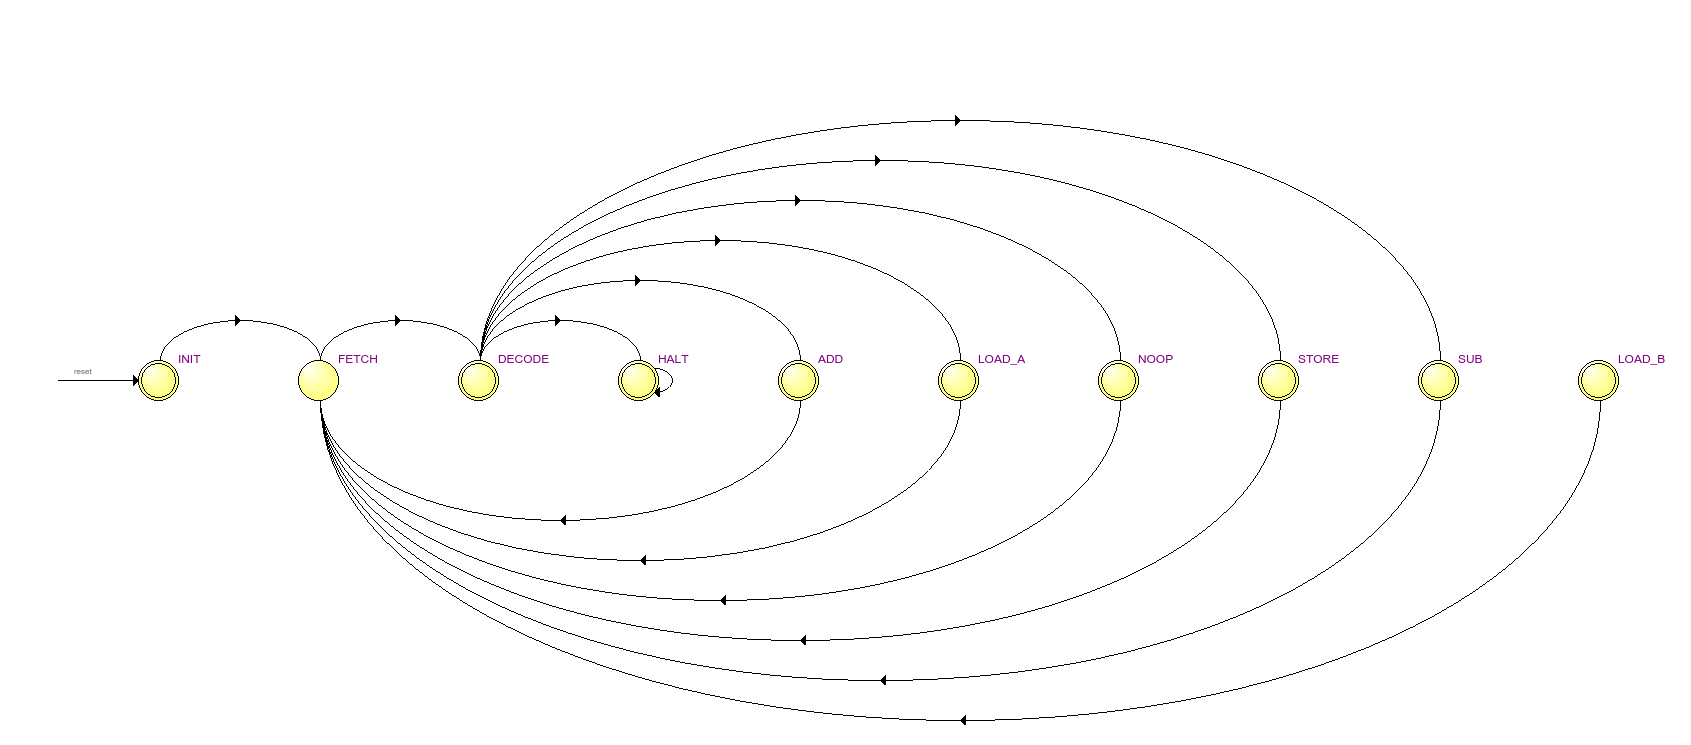
\includegraphics[width=\textwidth]{images/controller_rtl.png}
    \caption{Controller RTL View \label{fig:controller_rtl}}
\end{sidewaysfigure}

% subsection controller (end)

\FloatBarrier \subsection{Program Counter} % (fold)
\label{sub:program_counter}

The following observations correspond to the numbers in the \hyperref[sec:test_procedures]{Section \ref*{sec:test_procedures}} procedures for this part:

\begin{enumerate}
    \item The simulation using \emph{ModelSim} produced the output shown in \hyperref[fig:pc_output]{Figure \ref*{fig:pc_output}}.
    \item Sequantial values were generated when the count enable signal was high and the value was set to zero on a high reset signal.
\end{enumerate}

\begin{figure}[htbp]
    \begin{lstlisting}[numbers=none, basicstyle = \ttfamily\scriptsize]
# Time is          0 | Clock = 0 | Clear = 0 | O = 00
# Time is         10 | Clock = 1 | Clear = 0 | O = 01
# Time is         20 | Clock = 0 | Clear = 0 | O = 01
# Time is         30 | Clock = 1 | Clear = 0 | O = 02
# Time is         40 | Clock = 0 | Clear = 0 | O = 02
# Time is         50 | Clock = 1 | Clear = 0 | O = 03
# Time is         60 | Clock = 0 | Clear = 0 | O = 03
# Time is         70 | Clock = 1 | Clear = 0 | O = 04
# Time is         80 | Clock = 0 | Clear = 0 | O = 04
# Time is         90 | Clock = 1 | Clear = 0 | O = 05
# Time is        100 | Clock = 0 | Clear = 0 | O = 05
# Time is        110 | Clock = 1 | Clear = 0 | O = 05
# Time is        120 | Clock = 0 | Clear = 0 | O = 05
# Time is        130 | Clock = 1 | Clear = 0 | O = 05
# Time is        140 | Clock = 0 | Clear = 0 | O = 05
# Time is        150 | Clock = 1 | Clear = 0 | O = 05
# Time is        160 | Clock = 0 | Clear = 0 | O = 05
# Time is        170 | Clock = 1 | Clear = 0 | O = 05
# Time is        180 | Clock = 0 | Clear = 0 | O = 05
# Time is        190 | Clock = 1 | Clear = 0 | O = 05
# Time is        200 | Clock = 0 | Clear = 1 | O = 05
# Time is        210 | Clock = 1 | Clear = 1 | O = 00
# Time is        220 | Clock = 0 | Clear = 1 | O = 00
# Time is        230 | Clock = 1 | Clear = 1 | O = 00
# Time is        240 | Clock = 0 | Clear = 1 | O = 00
# Time is        250 | Clock = 1 | Clear = 1 | O = 00
# Time is        260 | Clock = 0 | Clear = 1 | O = 00
# Time is        270 | Clock = 1 | Clear = 1 | O = 00
# Time is        280 | Clock = 0 | Clear = 1 | O = 00
# Time is        290 | Clock = 1 | Clear = 1 | O = 00
    \end{lstlisting}
    \caption{Program Counter \emph{ModelSim} Output\label{fig:pc_output}}
\end{figure}

% subsection program_counter (end)

\FloatBarrier \subsection{Instruction Register} % (fold)
\label{sub:instruction_register}

The following observations correspond to the numbers in the \hyperref[sec:test_procedures]{Section \ref*{sec:test_procedures}} procedures for this part:

\begin{enumerate}
    \item The simulation using \emph{ModelSim} produced the output shown in \hyperref[fig:ir_output]{Figure \ref*{fig:ir_output}}.
    \item The register was loaded when the load enable signal was high and not when the load signal was low as expected.
\end{enumerate}

\begin{figure}[htbp]
    \begin{lstlisting}[numbers=none, basicstyle = \ttfamily\scriptsize]
# Time is          0 | input = 0000 | output = 0000
# Time is         20 | input = b0b0 | output = 0000
# Time is         30 | input = b0b0 | output = b0b0
# Time is         60 | input = d0d0 | output = b0b0
    \end{lstlisting}
    \caption{Instruction Register \emph{ModelSim} Output\label{fig:ir_output}}
\end{figure}

% subsection instruction_register (end)

\FloatBarrier \subsection{Processor} % (fold)
\label{sub:processor}

The following observations correspond to the numbers in the \hyperref[sec:test_procedures]{Section \ref*{sec:test_procedures}} procedures for this part:

\begin{enumerate}
    \item The simulation using \emph{ModelSim} produced the output shown in \hyperref[fig:processor_output]{Figure \ref*{fig:processor_output}}.
    \item  This output is inconsistent with that expected.
    The correct states are generated in sequence and correct register values are loaded, but the ALU does not generate proper output.
\end{enumerate}

\begin{sidewaysfigure}[htbp]
    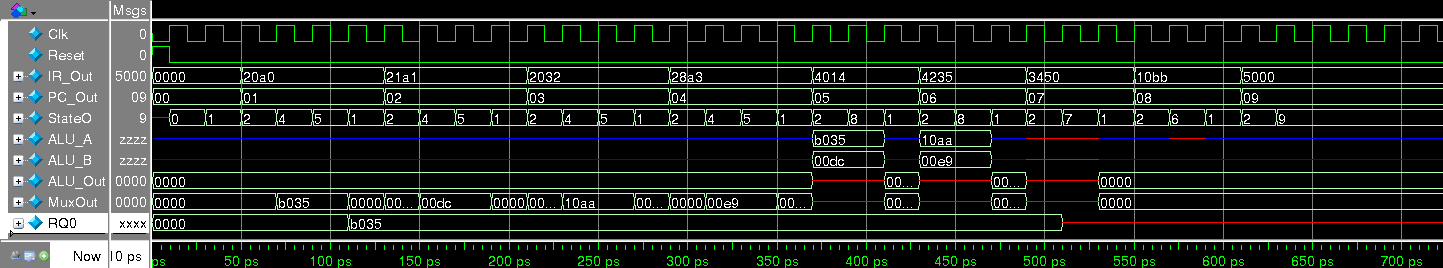
\includegraphics[width=\textwidth]{images/wave.png}
    \caption{Processor \emph{ModelSim} Output\label{fig:processor_output}}
\end{sidewaysfigure}

% subsection processor (end)

\FloatBarrier \subsection{Project} % (fold)
\label{sub:projects}

The following observations correspond to the numbers in the \hyperref[sec:test_procedures]{Section \ref*{sec:test_procedures}} procedures for this part:

\begin{enumerate}
    \item Compilation was successful, with the Flow Summary shown in \hyperref[lst:flow_summary]{Listing \ref*{lst:flow_summary}}.
    \item The project was downloaded to the DE2 board without errors.
    \item The displayed output was selectable as described in \hyperref[tab:display]{Table \ref*{tab:display}}.
    The program executed as expected with a final value of \verb|xBF1A| in register 0 as shown in \hyperref[fig:de2]{Figure \ref*{fig:de2}}.
\end{enumerate}

\lstinputlisting[basicstyle = \ttfamily\scriptsize, caption = \texttt{Flow Summary}, label = lst:flow_summary, numbers=none, keywords ={}]{flow_summary.rpt}

\FloatBarrier
\begin{figure}
    \includegraphics[width=\textwidth]{images/photo.png}
    \caption{DE2 Register Output\label{fig:de2}}
\end{figure}

% subsection projects (end)

% section test_results (end)